\section*{\hypertarget{talent}{Talents}}
\addcontentsline{toc}{subsection}{Talents}%
"Sweet Christmas, it's a talking turtle!" \\
\indent -- Bartz
\begin{center} 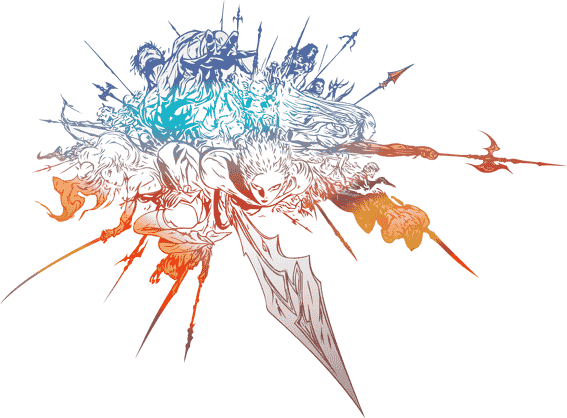
\includegraphics[width=1\columnwidth]{./art/images/ff14.png} \end{center}
%
Talents are non-combat related skills that a character is especially proficient with.
Every character starts the game with one talent and acquires a second one at \textbf{Level~6}, through his or her newly made experiences.
The GM may also allow characters to gain additional Talents under special circumstances.
Below, some Talents are shown that can be used as given, but the GM may also allow players to create their own Talents by using the given ones as examples. \\

\begin{description}[leftmargin=*]
	
\feat{Alchemist}
{
	After every successful battle against monsters you can spend a few minutes to create a \hyperlink{item}{Bomb Fragment}, \hyperlink{item}{Arctic Wind} or \hyperlink{item}{Lightning Gem} out of their remains. 
}

\feat{Archylte Hunter}
{
	You have \hyperlink{check}{Advantage} on all checks related to catching animals including hunting and fishing.
}

\feat{Blue Mage}
{
	You can quickly learn most simple non-combat skills by carefully observing someone proficient during the act for a while. 
	Such simple skills are for example cooking a meal or riding a \hyperlink{chocobo}{Chocobo}.
}

\feat{Calculator}
{
	Given enough time, you can solve any mathematical problem.
	Furthermore, you can make reliable numerical estimates, e.g. for various distances or the amount of people in a group.
}

\feat{Camping Again}
{
	While outside, you can spend an hour to build a comfortable shelter to spend the night out of materials found in nature.
}	
	
\feat{Carpenter}
{
	Given enough time and materials, you can create and repair any object that is mostly made out of wood,
	including sculptures, furniture and vehicles.
}

\pagebreak

\feat{Chemist}
{
	You can spend an hour to create a \hyperlink{item}{Potion} or a  \hyperlink{item}{Remedy} from ingredients found in nature or in stores.
}

\feat{Chocobo Sage}
{
	You can comfortably tame and build friendships with friendly animals and monsters like \hyperlink{chocobo}{Chocobos}.
}

\feat{Cid's Apprentice}
{
	Given enough time and materials you are able to repair any broken device or gadget. 
}

\feat{Conjurer}
{
	You can spend a few minutes to perform a ritual that creates an illusion of a character or an at most similarly sized monster or object.
	To understand that it is an illusion, a character either has to touch it or pass a DC~8 check.
}

\feat{Dedicated Driver}
{
	You are able to perfectly drive or navigate any vehicle including ships and airships. 
}
\feat{Doma's Enemy}
{
	You can spend an hour to create a potent poison out of materials found in nature or in stores.
	The poison is liquid, tasteless and odorless, so it can only be detected by experts such as yourself.
	A character that consumes the poison makes a DC~8 check and suffers \hyperlink{status}{KO} upon failure.
	Otherwise, he suffers \hyperlink{status}{Poison} for 3 rounds. 
}

\feat{Eyes Peeled}
{
	You are able to capture perfect images of scenes, landscapes and people as a painting or photograph.
}	

\feat{Excalipoor}
{
	Whenever you see an equipment piece, you can immediately understand its special effects.
	Furthermore, whenever you upgrade weapons and armor for your own use, it only costs you half as much Gil as usual.
}

\feat{Flower Girl} 
{
	You are able to identify any plant and know how to grow them even in very unfavorable conditions.
}

\feat{Gambler}
{
	You have \hyperlink{check}{Advantage} on all checks that involve in-game random events such as dice rolls or card draws.
}

\feat{Geomancer}
{
	You have \hyperlink{check}{Advantage} on all checks that require proficiency and experience related to nature, such as following tracks in a forest. 
}

\feat{Guardian Corps} 
{
	You do not suffer damage by falling from any height.
}

\feat{Haven't We Met Before}
{
	Whenever you meet a new character, you may declare that you have met them before.
	If you do so, the GM decides what kind of connection you have to that character.	
	You can only use this effect a total of 3 times in the entire adventure.
}

\pagebreak

\feat{Hope's Assistant} 
{
	Given any object or trace, you can determine its date and place of creation accurately.
}

\feat{King's Shield}
{
	You have \hyperlink{check}{Advantage} on all checks that mostly rely on strength such as lifting heavy objects or opening tight jar lids.
}

\feat{Lady Luck}
{
	Whenever you roll a total result of 2 on a check that you make outside of combat, you can redo the roll.
}

\feat{Leading Man}
{
	You have \hyperlink{check}{Advantage} on all checks that involve impressing or persuading someone through speech. 
}

\feat{Let's Mosey}
{
	You can perfectly imitate the behavior and mannerisms of a person that you have spent a few days of time with.
}

\feat{Llymlaen's Disciple}
{
	You never lose your way, even in locations that you are unfamiliar with.
	Moreover, you have no issues with reading maps or following given directions. 
}

\feat{Mognet}
{
	You can send telepathic messages to any person that you can see.
	If the recipient is further than 100u away from you, you have to pass a DC~7 check first.
}

\feat{O'aka XXIV}
{
	Whenever you are selling goods to someone who is willing to buy them, you can convince him to buy them at their original value despite being used.
}

\feat{Opera Floozy}
{
	You have \hyperlink{check}{Advantage} on all checks that involve acting, singing, dancing or performing in general.
}

\feat{Orator}
{
	Whenever you talk to a character that you know, you can spend a few minutes of time to motivate and inspire them.
	The character then has \hyperlink{check}{Advantage} on the next check that they perform.
}

\feat{Pharmacologist}
{
	Whenever you use an \hyperlink{item}{Item} outside of combat on yourself, you gain the following additional benefits: 
	if the Item increases your HP, you regain twice as much as usual. Otherwise, you regain 1d HP in addition to its usual effect. 
}

\feat{Scanner}
{
	While you are not combat, you can observe a character to immediately know their Level as well as their Job.
	You can also make a DC~8 check and if you succeed, you also know their Talents.
}

\pagebreak

\feat{Sceptic}
{
	You have \hyperlink{check}{Advantage} on all checks related to understanding whether someone is lying or withholding information.
}

\feat{Shrouded One} 
{
	You have \hyperlink{check}{Advantage} on all checks related to hiding or staying undetected.
}

\feat{Simdemehkiym}
{
	You are fluent in 2 languages and can learn new ones in a matter of days.
}

\feat{Skywatcher}
{
	You can accurately predict the weather in your current location for the next week.
}

\feat{Spira's Historian}
{
	You have knowledge on all important historical facts about the world.
	Furthermore, you have \hyperlink{check}{Advantage} on recollecting and making connections to more obscure historical events. 	 
}

\feat{Spoony Bard}
{
	You have perfectly mastered one music instrument of your choice.
	Furthermore, you can play any music piece on any music instrument to a convincing degree.
}

\feat{Starplayer}
{
	You are among the best in the world in one sport or game of your choice.
}

\feat{Strange Gourmand}
{
	You can spend an hour to prepare a tasty meal from almost anything that can be found in stores or in nature.
}

\feat{Tantalus Performer}
{
	You can use magic to create simple effects, including various voices and noises, small flames and gusts of wind.
}

\feat{Theologian}
{
	You have perfect knowledge on all religions in the world, including their deities, as well as their different customs and factions.
}

\feat{Thief's Caution}
{
	You have \hyperlink{check}{Advantage} on all checks related to noticing possible ambushes or hostile intentions of characters.
}

\feat{Walkthrough}
{
	You have \hyperlink{check}{Advantage} on all checks related to finding hidden locations and passages. 	 
}

\feat{Weaver}
{
	Given enough time and materials, you are able to create any kind of cloth or clothing.
}

\feat{Yin and Yang}
{
	While not in combat, you can meditate for a few minutes to gain the following benefit:
	Reduce your MP by an amount of your choice and increase your HP by the same amount.
}

\end{description}

\pagebreak